%%%%%%%%%%%%%%%%%%%%%%%%%%%%%%%%%%%%%%%%%%%%%%%%%%%%
\documentclass[fleqn,10pt,twocolumn]{AROB}

\usepackage[utf8]{inputenc}
\usepackage{amsmath}
\usepackage{xeCJK}
\usepackage{svg}
\setCJKmainfont{Hiragino Mincho ProN}

\title{可視カメラ 30fps 環境の PPG に最適化した\\
非対称サイン波モデル残差に基づく血圧推定}

\author{中澤 祐介${}^{1\dagger}$,南雲健人${}^{1}$,野澤昭雄${}^{1}$}
% The dagger symbol indicates the presenter.
\speaker{中澤 祐介}

\affils{${}^{1}$青山学院大学大学院理工学研究科 電気電子工学専攻\\
(Tel: 080-5326-3916; E-mail: nynynakazawa@gmail.com)\\
}

\abstract{%
スマートフォン可視カメラ由来の擬似PPGに対し、周波数分解に依存しない新規な血圧推定手法を提案する。30fpsという低サンプリングレート環境において、従来の周波数解析アプローチは高次高調波の正確な抽出が困難である。本研究では、既存の形態学的特徴量アプローチ(RTBP:RealTimeBloodPressure)をベースラインとして採用し、新規に提案する2つの手法を実装し、比較する。第一に、sin波フィットのパラメータ(振幅、位相、平均値)を直接特徴量として使用した線形回帰モデル(sinBP(M): sinBP(Model))である。第二に、生理学的に妥当な非対称サイン波モデルからの残差(歪み指標E)を特徴量として使用した3段階推定モデル(sinBP(D): sinBP(Distortion))である。sinBP(M)とsinBP(D)は、PPG波形の本質的な特性を抽出し、ノイズの影響を受けにくい安定した血圧推定を実現する。本研究の評価は、連続血圧計を参照として、30fps可視カメラのrPPG環境を使用した3つの異なる血圧推定手法(RTBP、sinBP(M)、sinBP(D))を比較し、新規手法の優位性を検証する。
}

\keywords{%
血圧推定、光電容積脈波、スマートフォン、非対称サイン波モデル、歪み指標
}

\begin{document}

\maketitle

%-----------------------------------------------------------------------

\section{序論}

\subsection{背景と動機}

連続的な非侵襲血圧モニタリングの需要は、高血圧や心血管疾患の早期発見・管理において極めて高い\cite{ref1,ref2}。従来の血圧測定は上腕カフを用いた間欠的な測定が主流であるが、日常生活における連続的な血圧変動を捉えるには不十分である。近年、スマートフォンの可視カメラを用いた光電容積脈波(PPG: Photoplethysmography)による血圧推定が注目されている。PPGは皮膚表面の血流変化を光の吸収変化として検出する技術であり、専用デバイスを必要とせず、スマートフォンだけで測定可能という利点がある\cite{ref3}。

しかし、スマートフォン可視カメラを用いたPPG測定には重大な制約が存在する。まず、フレームレートが30fpsと低く、従来のPPGセンサー(数百Hz)と比較して時間分解能が低い。次に、可視光を用いるため、周囲の照明条件の変動やノイズの影響を受けやすい。さらに、カメラの自動露出制御(AEC)や自動ゲイン制御(AGC)により、信号の動的範囲が制限される。これらの制約により、従来の高調波比・THD(Total Harmonic Distortion)・A$_2$/A$_1$等の周波数分解を前提とした手法は、位相ゆらぎや照明変動に対して脆弱である\cite{ref4,ref5}。

\subsection{従来研究の課題と線形回帰モデルの理論的背景}

\subsubsection{従来研究の課題}

従来のPPGベースの血圧推定手法は、主に以下のアプローチに分類される:

\begin{enumerate}
\item \textbf{形態学的特徴量アプローチ}: 波形の形状特徴(ピーク値、谷値、Time-To-Peak、勾配など)を抽出し、線形回帰や機械学習により血圧を推定する手法\cite{ref6}。しかし、30fpsという低サンプリングレートでは、波形の微細な形状変化を捉えることが困難である。

\item \textbf{周波数解析アプローチ}: FFTやウェーブレット変換により周波数領域の特徴を抽出する手法。高調波比(A$_2$/A$_1$)やTHDを特徴量として使用する\cite{ref7}。しかし、30fpsではナイキスト周波数が15Hzと低く、高次高調波の正確な抽出が困難である。また、位相ゆらぎや照明変動により、周波数特性が不安定になる。

\item \textbf{機械学習アプローチ}: 深層学習やサポートベクターマシンを用いて、生波形から直接血圧を推定する手法\cite{ref8}。しかし、大量の学習データが必要であり、30fpsという低FPS条件での汎化性能が不十分である。
\end{enumerate}

\subsubsection{線形回帰モデルを用いる理論的背景}

PPG信号から血圧を推定する際、PPGの特徴量と血圧値の間に線形関係が存在することが多くの先行研究で示されている。例えば、PPG信号の形態特徴量を用いた血管年齢の推定において、部分的最小二乗(PLS)回帰を適用することで、血管年齢の推定が可能であることが報告されている\cite{ref9}。また、PPG信号の形状特徴量と血圧値の間に一定の相関関係が認められており、線形回帰モデルを用いることで血圧の推定が可能であると示されている\cite{ref6,ref10}。

これらの先行研究の知見に基づき、本研究では以下の3つの手法において、それぞれ異なる特徴量を用いた線形回帰モデルを採用する。特に、PPGから抽出される特徴量は互いに強い相関(多重共線性)を持つことが多いため、通常の最小二乗法(OLS)ではなく、正則化項を加えた\textbf{Ridge回帰}を採用する。Ridge回帰は、係数の大きさを抑制することで過学習を防ぎ、ノイズの多い環境や特徴量間の相関が高い場合でも安定した推定を実現できる手法として、本分野でも広く用いられている\cite{ref8,ref12}。

\textbf{RTBP(既存手法)}: 形態学的特徴量(振幅A、心拍数HR、相対Time-To-Peak)と血圧の間には、生理学的に説明可能な線形関係が存在することが報告されている\cite{ref6}。特に、PPG振幅は血管の拡張能を反映し、心拍数は循環動態を反映するため、これらを組み合わせることで血圧推定が可能である。

\textbf{sinBP(M)(新規手法)}: sin波フィットにより得られるパラメータ(振幅A、平均値Mean、位相Phi)は、PPG波形の本質的な特性を抽出したものである。具体的には、\textbf{振幅A}は拍動ごとの血液量変化(AC成分)を反映し、血管の伸展性や脈圧と関連する\cite{ref11}。\textbf{平均値Mean}は組織血液量(DC成分)を反映し、自律神経活動や静脈還流の状態を示す\cite{ref11}。\textbf{位相Phi}は脈波の到達タイミングを示し、血管硬化度や血圧と相関する脈波伝播速度(PWV)の情報を内包している\cite{ref12}。これらのパラメータを特徴量として用いることで、ノイズの影響を受けにくい安定した血圧推定が可能になると予想される。

\textbf{sinBP(D)(新規手法)}: 非対称サイン波モデルからの残差(歪み指標E)は、実測波形が理想的な生理学的モデルからどれだけ外れているかを定量化する。この残差は、血管の硬さや動脈硬化の進行と関連することが知られており\cite{ref13,ref14}、血圧推定に有効な特徴量となると予想される。特に、Eと振幅Aの平方根の積(Stiffness\_sin = E$\sqrt{A}$)は、血管の拡張能と波形の歪みを組み合わせた合成指標として、血圧推定に独立寄与を持つと予想される。

これらの理論的背景に基づき、本研究では3つの手法それぞれにおいて、Ridge回帰モデルを用いて血圧推定を行うことを提案する。

\subsection{sin近似を選んだ理由}

本研究では、30fpsという低FPS・高ノイズ環境において、周波数分解に依存しない手法としてsin波近似を採用した。その理由は以下の通りである。

第一に、\textbf{周波数分解の制約}である。30fpsではナイキスト周波数が15Hzと低く、高次高調波の正確な抽出が困難である。従来の高調波比(A$_2$/A$_1$)やTHD(Total Harmonic Distortion)を特徴量とする手法は、位相ゆらぎや照明変動により周波数特性が不安定になる。これに対し、sin波近似は周波数領域への変換を必要とせず、時間領域で直接モデルを構築するため、30fpsという低FPS環境でも安定した特徴抽出が可能である。

第二に、\textbf{生理学的妥当性}である。PPG波形は心臓の拍動に伴う動脈の拡張・収縮を反映しており、基本的には周期的な一峰波形である。生理学的には、収縮期(心臓が血液を送り出す期間)は拡張期(心臓が血液をためる期間)よりも短く、典型的には収縮期が周期の約1/3、拡張期が約2/3である。本研究では、この非対称性を反映した非対称サイン波モデルを採用し、実装では1拍遅延処理により前の拍の実測データから収縮期/拡張期比率を自動計算することで、各拍ごとに動的にモデルを構築する。これにより、PPG波形の生理学的特性を適切に表現できる。

第三に、\textbf{ノイズに対する頑健性}である。30fpsという低サンプリングレートでは、波形の微細な形状変化を捉えることが困難であり、形態学的特徴量アプローチはノイズの影響を受けやすい。これに対し、sin波近似は1拍全体をモデル化するため、局所的なノイズの影響を受けにくく、より安定した特徴抽出が可能である。

第四に、\textbf{実装容易性と計算効率}である。sin波近似は少数のパラメータ(振幅、位相、平均値)で1拍波形を表現できるため、計算コストが低く、リアルタイム処理に適している。また、位相はデータ駆動で自動整合されるため、手動調整が不要である。

これらの理由から、本研究では周波数分解に依存せず、生理学的に妥当な非対称サイン波モデルを基準とし、基準からの外れ(最小モデル残差)を一次特徴化するアプローチを採用した。

\subsection{本研究の目的と評価}

本研究では、3つの異なる血圧推定手法を実装し、比較する。第一に、形態学的特徴量(振幅、心拍数、相対Time-To-Peak)のみを使用した線形回帰モデル(RTBP: RealtimeBP)である。第二に、sin波フィットのパラメータ(振幅、位相、平均値)を直接使用した線形回帰モデル(sinBP(M): sinBP(Model))である。第三に、非対称サイン波モデルからの残差(歪み指標E)を特徴量として使用した3段階推定モデル(sinBP(D): sinBP(Distortion))である。

本研究の目的は以下の2点である:

\begin{enumerate}
\item \textbf{波形評価}: パルスオキシメーターの参照波形とrPPG実波形、非対称サイン波モデルによる近似波を時間同期させ、MAPE(Mean Absolute Percentage Error)により波形の近似精度を評価する。これにより、非対称サイン波モデルが30fpsという低FPS環境において、実波形をどれだけ正確に近似できるかを定量化する。

\item \textbf{血圧推定精度の比較}: 連続血圧計を参照として、3つの異なる血圧推定手法(RTBP、sinBP(M)、sinBP(D))を比較し、非対称サイン波モデルを用いた手法(sinBP(M)、sinBP(D))が本環境(30fps可視カメラ)において、従来の形態学的特徴量のみを用いた手法(RTBP)と比較して、本当に精度が高くなるのかを検証する。
\end{enumerate}

\subsection{本研究の貢献}

本研究の主な貢献は以下の4点である:

\begin{enumerate}
\item \textbf{sinBP(M)の新規性}: 非対称サイン波モデルへのフィットにより得られるパラメータ(振幅、位相、平均値)を特徴量として用いることで、30fps環境においてもノイズの影響を受けにくい安定した血圧推定を実現する新規手法を提案する。先行研究で示されているPPG波形のDC成分と血圧の相関\cite{ref11}、および位相情報と血管特性の関連\cite{ref12}を理論的背景として、線形回帰モデルを適用する。

\item \textbf{sinBP(D)の新規性}: 生理学的に妥当な非対称サイン波モデルを定義し、モデルからの残差(歪み指標E)と血管硬さ指標(Stiffness\_sin = E$\sqrt{A}$)を特徴量として用いる新しい推定枠組みを提案する。非対称性は1拍遅延処理により実測データから自動計算される。この残差は、血管の硬さや動脈硬化の進行と関連することが知られており\cite{ref13}、血圧推定に有効な特徴量となる。

\item \textbf{IBI同期(拍ごとにT=IBI)かつピーク整合(位相探索)による比較可能な正規化}: 各拍のIBI(Inter-Beat Interval)に同期させ、データ駆動の位相探索により理想波のピークを実測ピークに整合させることで、拍ごとの変動を考慮した正規化を実現する。

\item \textbf{同一データ・同一前処理での対照実験計画}: 既存手法(RTBP)と新規手法(sinBP(M)、sinBP(D))を同一データ・同一前処理で比較し、各手法の特徴量の寄与を定量化する。特に、非対称サイン波モデルのパラメータを用いた手法(sinBP(M))と、同モデルの残差を用いた手法(sinBP(D))の両方を比較することで、新規手法の優位性を検証する。
\end{enumerate}

%-----------------------------------------------------------------------

\section{手法}

\subsection{データ取得と前処理の概要}

本研究では、スマートフォンの可視カメラ(30fps)からPPG信号を取得し、3つの異なる手法で血圧を推定する。データ取得は、YUV画像からU値を元にGreen値を抽出し、指先の周辺領域の平均値を計算することで、動脈の拍動による血流変化を検出する。各拍ごとにピーク検出を行い、IBI(Inter-Beat Interval)を計算する。IBIの範囲は0.25秒~1.2秒(50~240 BPM相当)に制限し、この範囲外の値は外れ値として除外する。

本システムの処理フローをFig. \ref{fig:app_flow}に示す。

\begin{figure}[t]
\centering
% 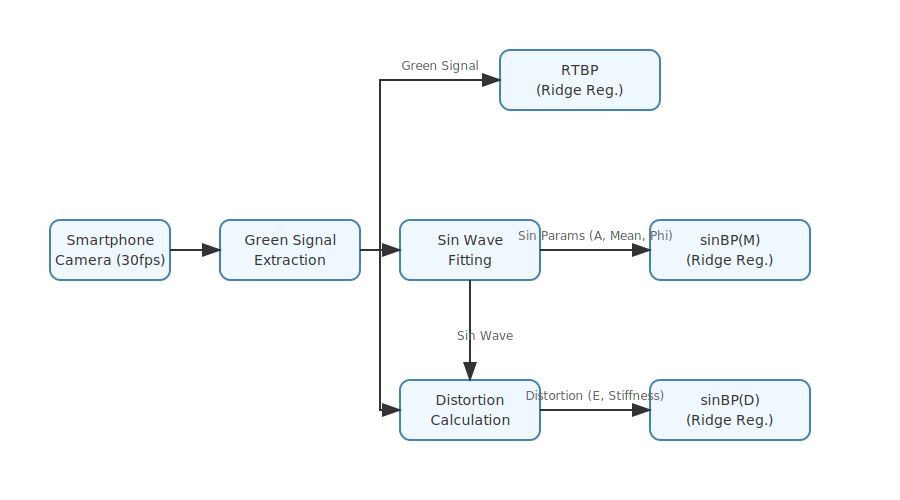
\includegraphics[width=\linewidth]{figures/app_flow.svg}
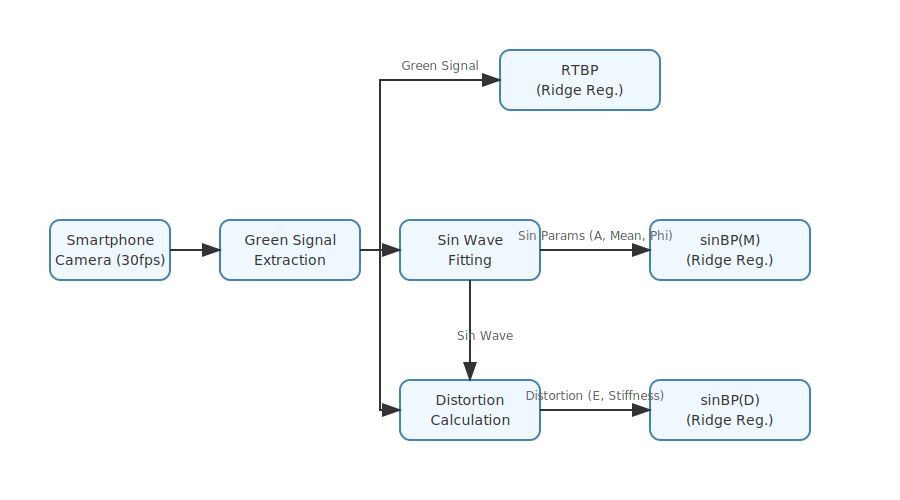
\includegraphics[width=\linewidth]{figures/app_flow.png}
\caption{Processing flow of the proposed smartphone-based blood pressure estimation.}
\label{fig:app_flow}
\end{figure}

\subsection{非対称サイン波モデルについて}

本研究では、提案手法であるsinBP(M)とsinBP(D)において、生理学的に妥当な非対称サイン波モデルを使用する。PPG波形は、心臓の拍動に伴う動脈の拡張・収縮を反映している。生理学的には、収縮期(心臓が血液を送り出す期間)は拡張期(心臓が血液をためる期間)よりも短く、典型的には収縮期が周期の約1/3、拡張期が約2/3である\cite{guyton}。この非対称性を反映するため、本研究では以下の非対称サイン波モデルを定義する:

\begin{equation}
s(t) = \text{mean} + A \cdot s_{\text{norm}}(t)
\label{eq:asymmetric_model}
\end{equation}

\begin{equation}
s_{\text{norm}}(t) = \frac{1 + \cos(\theta(t) + \phi_0)}{2}
\label{eq:asymmetric_norm}
\end{equation}

\begin{equation}
\theta(t) = \begin{cases}
\frac{3\pi}{2} \cdot \frac{t'}{T} & (0 \leq t' \leq \alpha T) \\
\pi + 3\pi \cdot \frac{t' - \alpha T}{T} & 
(\alpha T < t' \leq T)
\end{cases}
\label{eq:asymmetric_theta}
\end{equation}

ここで、$A$は振幅、meanは平均値、$T$は周期(IBI)である。$t' = (t - \tau^*) \bmod T$は1拍内の位相時間、$\phi_0$は小さな位相シフト、$\tau^*$は各拍ごとにピーク位置を整合させるためのパラメータである。また、$\alpha$は収縮期の割合を表すパラメータであり、初期値として$\alpha \approx 1/3$(拡張期は$1-\alpha \approx 2/3$)と仮定する。

実装では、1拍遅延処理により前の拍の実測データから収縮期/拡張期比率を自動計算し、その比率に基づいて動的にモデルパラメータ$\alpha$を決定する。デフォルト値として、ピーク→谷が周期の約2/3、谷→次ピークが約1/3となる比率を使用するが、各拍ごとに実測データから計算された動的な比率が用いられる。

\subsubsection{sinBP(M)におけるモデルの利用}

sinBP(M)では、上記の非対称サイン波モデルを実測データに適用し、得られたモデルパラメータ(振幅$A$、平均値mean、位相$\phi$)を血圧推定の特徴量として直接使用する。パラメータ抽出には、安定性を重視してDFT(離散フーリエ変換)ベースの手法を用いる。

\subsubsection{sinBP(D)における歪み指標と血管硬さ指標}

sinBP(D)では、モデルパラメータに加えて、実測波形とモデル波形の残差に着目する。1拍分の実測データ$x[n]$($N$点)に対して非対称サイン波モデル$s[n]$をフィットし、その残差RMS誤差を歪み指標$E$として計算する。なお、本実装では心拍数によるサンプル数の変動を正規化するため、各拍の実測データを$N=64$点にリサンプリングしてから計算を行う:

\begin{equation}
E = \sqrt{\frac{1}{N} \sum_{n=1}^{N} (x[n] - s[n])^2}
\label{eq:distortion}
\end{equation}

歪み指標$E$は、実測波形が理想的な非対称サイン波モデルからどれだけ外れているかを定量化する。血管硬化に伴いPPG波形が変化し、反射波の影響等で歪みが生じることは先行研究で報告されている\cite{ref6,ref13}。したがって、$E$が大きいほど波形の歪みが大きく、血管の硬さや動脈硬化の進行を示唆すると考えられる。

さらに、歪み指標$E$と振幅$A$の平方根の積を、血管硬さ指標Stiffness\_sinとして定義する:

\begin{equation}
\text{Stiffness}_{\text{sin}} = E \sqrt{A}
\label{eq:stiffness}
\end{equation}

PPG振幅は血管の伸展性(コンプライアンス)を反映し\cite{ref3}、波形歪みは動脈スティフネスを反映する\cite{ref14}ことから、この指標はこれらを組み合わせることで、血管の硬さをより包括的に評価する合成指標となる。従来のAI(Augmentation Index)と比較して、30fpsという低FPS条件でも安定して計算できる利点がある。

\subsection{3つの血圧推定手法}

本研究では、3つの異なる血圧推定手法を実装し、比較する。第一に、既存の形態学的特徴量アプローチ(RTBP)をベースラインとして採用する。第二に、新規に提案する非対称サイン波モデルパラメータベースの手法(sinBP(M))を実装する。第三に、新規に提案する非対称サイン波モデル残差ベースの手法(sinBP(D))を実装する。

\subsubsection{手法1: RTBP (RealtimeBP) - 既存手法(ベースライン)}

RTBPは、PPG波形の形態学的特徴量のみを使用した線形回帰モデルである。この手法は、先行研究で報告されている標準的なアプローチであり\cite{ref6,ref10}、本研究ではベースライン手法として採用する。

\textbf{理論的背景}: PPG波形の形態学的特徴量(振幅、心拍数、Time-To-Peak)と血圧の間には、生理学的に説明可能な線形関係が存在することが報告されている\cite{ref6}。特に、PPG振幅は血管の拡張能を反映し、心拍数は循環動態を反映するため、これらを組み合わせることで血圧推定が可能である。

\textbf{特徴量}:
\begin{itemize}
\item $A$: 振幅(谷→山の振幅)
\item HR: 心拍数(60000.0 / IBI)
\item V2P\_relTTP: 谷→山の相対Time-To-Peak(IBIに対する相対的な時間)
\item P2V\_relTTP: 山→谷の相対Time-To-Peak
\end{itemize}

\textbf{推定式}:
\begin{equation}
\begin{split}
\text{SBP} &= C_0 + C_1 \cdot A + C_2 \cdot \text{HR} \\
&\quad + C_3 \cdot \text{V2P\_relTTP} + C_4 \cdot \text{P2V\_relTTP}
\end{split}
\label{eq:rtbp_sbp}
\end{equation}

\begin{equation}
\begin{split}
\text{DBP} &= D_0 + D_1 \cdot A + D_2 \cdot \text{HR} \\
&\quad + D_3 \cdot \text{V2P\_relTTP} + D_4 \cdot \text{P2V\_relTTP}
\end{split}
\label{eq:rtbp_dbp}
\end{equation}

\textbf{係数}: 学習データからRidge回帰により決定される。

\textbf{制約}: SBPは60~200 mmHg、DBPは40~150 mmHgの範囲に制限する。

\subsubsection{手法2: sinBP(M) (sinBP(Model)) - 新規手法}

sinBP(M)は、本研究で新規に提案する手法であり、非対称サイン波モデルへのフィットにより得られるパラメータ(振幅、位相、平均値)を直接特徴量として使用した線形回帰モデルである。

\textbf{理論的背景と新規性}: 従来の形態学的特徴量アプローチは、30fpsという低サンプリングレートでは波形の微細な形状変化を捉えることが困難である。これに対し、sinBP(M)では、1拍分のデータに対して非対称サイン波モデルをフィットし、そのパラメータを特徴量として使用する。モデルフィットにより得られるパラメータは、PPG波形の本質的な特性を抽出したものであり、ノイズの影響を受けにくい。先行研究では、PPG波形のDC成分(平均値)が血圧と相関することが示されており\cite{ref11}、また位相情報は血管特性を反映することが知られている\cite{ref12}。これらの知見に基づき、非対称サイン波モデルのパラメータを特徴量として用いることで、30fps環境においても安定した血圧推定が可能になると予想される。

\textbf{非対称サイン波モデル}: 1拍分のデータに対して、前述の非対称サイン波モデル(式\ref{eq:asymmetric_model})を適用する。

\begin{equation}
s(t) = \text{mean} + A \sin\left(\frac{2\pi t}{T} + \phi\right)
\label{eq:sin_model_m}
\end{equation}

ここで、$A$は振幅、meanは平均値、$\phi$は位相、$T$は周期(IBI)である。各拍ごとにIBIに同期させ、データ駆動の位相探索により理想波のピークを実測ピークに整合させることで、拍ごとの変動を考慮した正規化を実現する。

\textbf{特徴量}:
\begin{itemize}
\item $A$: 振幅(モデルフィットから取得)
\item HR: 心拍数(60000.0 / IBI)
\item Mean: 平均値(モデルフィットから取得、DC成分)
\item $\Phi$: 位相(モデルフィットから取得)
\end{itemize}

\textbf{推定式}:
\begin{equation}
\begin{split}
\text{SBP} &= \alpha_0 + \alpha_1 \cdot A + \alpha_2 \cdot \text{HR} \\
&\quad + \alpha_3 \cdot \text{Mean} + \alpha_4 \cdot \Phi
\end{split}
\label{eq:sinbp_m_sbp}
\end{equation}

\begin{equation}
\begin{split}
\text{DBP} &= \beta_0 + \beta_1 \cdot A + \beta_2 \cdot \text{HR} \\
&\quad + \beta_3 \cdot \text{Mean} + \beta_4 \cdot \Phi
\end{split}
\label{eq:sinbp_m_dbp}
\end{equation}

\textbf{係数}: 学習データからRidge回帰により決定される。

\textbf{制約}: SBPは60~200 mmHg、DBPは40~150 mmHgの範囲に制限する。

\subsubsection{手法3: sinBP(D) (sinBP(Distortion)) - 新規手法}

sinBP(D)は、本研究で新規に提案する手法であり、非対称サイン波モデルからの残差(歪み指標$E$)を特徴量として使用した3段階推定モデルである。この手法は、生理学的に妥当な非対称サイン波モデルを基準とし、基準からの外れを定量化することで、より高精度な血圧推定を実現する。

\textbf{理論的背景と新規性}: 非対称サイン波モデルからの残差(歪み指標$E$)は、実測波形が理想的な生理学的モデルからどれだけ外れているかを定量化する。この残差は、血管の硬さや動脈硬化の進行と関連することが知られており\cite{ref13,ref14}、血圧推定に有効な特徴量となると予想される。特に、$E$と振幅$A$の平方根の積(Stiffness\_sin = $E\sqrt{A}$)は、血管の拡張能と波形の歪みを組み合わせた合成指標として、血圧推定に独立寄与を持つと予想される。従来のAI(Augmentation Index)と比較して、30fpsという低FPS条件でも安定して計算できる利点がある。

\textbf{非対称サイン波モデル}: 生理学的には、収縮期(心臓が血液を送り出す期間)は拡張期(心臓が血液をためる期間)よりも短く、典型的には収縮期が周期の約1/3、拡張期が約2/3である。この非対称性を反映した非対称サイン波モデルを定義する。実装では、1拍遅延処理により前の拍の実測データから収縮期/拡張期比率を自動計算し、実測値に基づいて動的にモデルを構築する。デフォルト値として、収縮期が周期の約1/3、拡張期が約2/3となる比率を使用するが、各拍ごとに実測データから計算された動的な比率が用いられる。

\textbf{特徴量}:
\begin{itemize}
\item $A$: 振幅(モデルフィットから取得)
\item HR: 心拍数(60000.0 / IBI)
\item V2P\_relTTP: 谷→山の相対Time-To-Peak
\item P2V\_relTTP: 山→谷の相対Time-To-Peak
\item Stiffness\_sin: $E\sqrt{A}$(歪み指標×振幅の平方根、血管硬さ指標)
\item $E$: 歪み指標(非対称サイン波モデルからのRMS誤差)
\end{itemize}

\textbf{推定式(3段階推定)}:

3段階推定により、各特徴量の寄与を段階的に評価する。第1段では基本的な特徴量(振幅$A$、心拍数HR)のみを使用し、第2段で血管特性(相対TTP、Stiffness\_sin)を追加し、第3段で歪み指標$E$を追加する。

【第1段: ベースBP計算】
\begin{equation}
\text{SBP}_{\text{base}} = \text{ALPHA}_0 + \text{ALPHA}_1 \cdot A + \text{ALPHA}_2 \cdot \text{HR}
\label{eq:sinbp_d_sbp_base}
\end{equation}

\begin{equation}
\text{DBP}_{\text{base}} = \text{BETA}_0 + \text{BETA}_1 \cdot A + \text{BETA}_2 \cdot \text{HR}
\label{eq:sinbp_d_dbp_base}
\end{equation}

【第2段: 血管特性補正】
\begin{equation}
\begin{split}
\text{SBP}_{\text{Distortion} &= \text{SBP}_{\text{base}} \\
&\quad + \text{ALPHA}_3 \cdot \text{V2P\_relTTP} \\
&\quad + \text{ALPHA}_4 \cdot \text{P2V\_relTTP} \\
&\quad + \text{ALPHA}_5 \cdot \text{Stiffness}_{\text{sin}}
\end{split}
\label{eq:sinbp_d_sbp_model}
\end{equation}

\begin{equation}
\begin{split}
\text{DBP}_{\text{model}} &= \text{DBP}_{\text{base}} \\
&\quad + \text{BETA}_3 \cdot \text{V2P\_relTTP} \\
&\quad + \text{BETA}_4 \cdot \text{P2V\_relTTP} \\
&\quad + \text{BETA}_5 \cdot \text{Stiffness}_{\text{sin}}
\end{split}
\label{eq:sinbp_d_dbp_model}
\end{equation}

【第3段: 歪み補正】
\begin{equation}
\text{SBP} = \text{SBP}_{\text{Distortion} + \text{ALPHA}_6 \cdot E
\label{eq:sinbp_d_sbp_final}
\end{equation}

\begin{equation}
\text{DBP} = \text{DBP}_{\text{model}} + \text{BETA}_6 \cdot E
\label{eq:sinbp_d_dbp_final}
\end{equation}

\textbf{係数}: 学習データからRidge回帰により決定される。

\textbf{制約}: SBP $\geq$ DBP + 10、SBPは60~200 mmHg、DBPは40~150 mmHgの範囲に制限する。

\subsection{前処理と正規化の概要}

各手法において、以下の前処理を実施する:

\begin{itemize}
\item \textbf{ピーク検出}: 移動窓最大値検出によりピークを検出し、不応期を設ける。
\item \textbf{ビート切り出し}: 現在ピークから次ピークまでを1拍として切り出す。周期$T$はIBIに等しい。
\item \textbf{時間正規化}: sinBP(M)とsinBP(D)では、各拍を固定長($N=64$点)にリサンプリングする。RTBPは形態学的特徴量のみを使用するため、時間正規化は不要である。
\item \textbf{ピーク整合}: sinBP(M)とsinBP(D)では、各拍で位相探索により理想波のピークを実測ピークに一致させる。これにより、拍ごとの位相変動を考慮した正規化を実現する。
\item \textbf{外れ値抑制}: IBI・振幅・テンポラルジャンプに基づくルールベース除外を実施する。IBIが0.25秒~1.2秒の範囲外、振幅が前回の30\%以上変化、生理学的に妥当でない値は外れ値として除外する。
\end{itemize}

%-----------------------------------------------------------------------

\section{実験計画}

\subsection{データ取得プロトコル}

\subsubsection{環境設定}
\begin{itemize}
\item \textbf{デバイス}: Google Pixel 8 フロント可視カメラ(30fps)
\item \textbf{測定方式}: 指腹接触方式(第2指)
\item \textbf{照明条件}: 室内 400 lux
\end{itemize}

\subsubsection{参照値}
\begin{itemize}
\item \textbf{参照デバイス1}: 指先カフ(第3指)で実時間PPGを光学式パルスオキシメーター(IWS920-DEV 分解能409.6Hz)で同時計測
\item \textbf{参照デバイス2}: 指先カフ(第3指/第4指)で実時間血圧を連続血圧計(CNAP-Monitor 分解能1000Hz 臨床グレード)で同時計測
\item \textbf{測定条件}: 測定間隔・体位・安静時間を統一
\end{itemize}

\subsubsection{被験者}
\begin{itemize}
\item \textbf{被験者}: 20~23歳の健康な成人男性5名
\item \textbf{除外条件}: 不整脈重度等
\item \textbf{試行回数}: 各被験者につき3回ずつ計測
\end{itemize}

\subsubsection{倫理}
同意取得・匿名化・暗号化保存を実施する。

\subsection{波形評価実験}

\subsubsection{評価目的}

本研究では、スマートフォン可視カメラから取得したPPG波形が、高サンプリングレートの参照波形(409.6Hz)とどれだけ一致するかを評価することで、30fpsという低サンプリングレート環境における波形の品質を検証する。特に、生のGreenチャンネル(30Hz)と非対称サイン波モデルにより生成されたsinWaveチャンネル(30Hz)の両方を評価し、モデル近似が波形の本質的な特性を保持しているかを検証する。

\subsubsection{データ取得と前処理}

参照波形として、指先PPGセンサーから取得した高サンプリングレート(409.6Hz)のPPG波形を使用する。スマートフォン側の波形として、可視カメラから取得したGreenチャンネル(生のrPPG信号)と、非対称サイン波モデルにより生成されたsinWaveチャンネルを評価対象とする。

前処理として、参照波形にはアンチエイリアシングフィルタ(Butterworthローパスフィルタ、カットオフ周波数15 Hz)を適用し、30 Hzへのダウンサンプリングに伴う折り返し雑音を除去する。両波形に対して、修正Zスコア(MADベース)による外れ値除去を実施し、その後、振幅を共通のレンジ(0-10)に正規化する。

\subsubsection{時間同期とスケーリング}

参照波形をスマートフォン側の時間軸(30 Hz)に線形補間により整列させる。その後、参照波形とスマートフォン波形の振幅レンジを共通化するため、参照波形の最小値・最大値に合わせてスマートフォン波形を線形変換する(スケーリング)。これにより、振幅の絶対値の違いを排除し、波形の形状の一致度を評価できる。

\subsubsection{評価指標}

時間同期・スケーリング後の波形に対して、以下の指標を計算する:

\begin{itemize}
\item \textbf{MAPE(Mean Absolute Percentage Error)}: 正規化スケール幅(10)に対する平均絶対誤差の割合
\item \textbf{MAE(Mean Absolute Error)}: 平均絶対誤差
\item \textbf{RMSE(Root Mean Squared Error)}: 二乗平均平方根誤差
\item \textbf{Bias}: 平均誤差(推定値 - 参照値)
\item \textbf{相関係数}: 波形の形状の一致度を評価
\end{itemize}

これらの指標により、波形の振幅精度(MAE、RMSE)、系統誤差(Bias)、形状の一致度(相関係数)を包括的に評価する。

\subsection{血圧推定精度の比較実験}

本研究では、連続血圧計を参照として、3つの血圧推定手法の精度を比較する。全手法が同じ拍列・同じ正規化系列を入力する前提で比較し、学習/検証の分割は完全共通とする。これにより、各手法の特徴量の寄与を公平に評価できる。

\subsubsection{3手法の比較}

3つの異なる血圧推定手法(RTBP、sinBP(M)、sinBP(D))を比較する:
\begin{itemize}
\item \textbf{RTBP}: 形態学的特徴量のみを使用した手法(ベースライン)
\item \textbf{sinBP(M)}: 非対称サイン波モデルのパラメータを直接使用した手法
\item \textbf{sinBP(D)}: 非対称サイン波モデルの残差(歪み指標$E$)を用いた手法
\end{itemize}

\subsubsection{アブレーション研究}

3手法の各要素の寄与を定量化する。

\textbf{RTBPのアブレーション}:
\begin{enumerate}
\item[(i)] $A$・HR のみ: ベースライン
\item[(ii)] + V2P\_relTTP: 谷→山の相対TTPの寄与
\item[(iii)] + P2V\_relTTP: 山→谷の相対TTPの寄与
\end{enumerate}

\textbf{sinBP(M)のアブレーション}:
\begin{enumerate}
\item[(i)] $A$・HR のみ: ベースライン
\item[(ii)] + Mean: 平均値の寄与
\item[(iii)] + $\Phi$: 位相の寄与
\end{enumerate}

\textbf{sinBP(D)のアブレーション}:
\begin{enumerate}
\item[(i)] $A$・HR のみ: ベースライン
\item[(ii)] + V2P\_relTTP: 谷→山の相対TTPの寄与
\item[(iii)] + P2V\_relTTP: 山→谷の相対TTPの寄与
\item[(iv)] + Stiffness\_sin($E\sqrt{A}$): 血管硬さ指標の寄与
\item[(v)] + $E$: 歪み指標の重み付けによる寄与
\end{enumerate}

\subsection{検証設計・統計計画}

\subsubsection{データ分割}

時系列データとしての特性を考慮し、\textbf{TimeSeriesSplit}(時系列交差検証)を採用する。これは、データを時間の順序に従って分割し、過去のデータで学習したモデルを用いて未来のデータを予測する検証方法である。これにより、実運用に近い形での汎化性能を評価する。分割数は5分割とする。

\subsubsection{評価指標}

血圧推定の精度を評価するため、以下の指標を計算する:

\begin{itemize}
\item \textbf{MAE(Mean Absolute Error)}: 平均絶対誤差(mmHg)
\item \textbf{RMSE(Root Mean Squared Error)}: 二乗平均平方根誤差(mmHg)
\item \textbf{MAPE(Mean Absolute Percentage Error)}: 平均絶対パーセント誤差(\%)
\item \textbf{MD(Mean Difference)}: 平均誤差(推定値 - 参照値、mmHg)
\item \textbf{SD(Standard Deviation)}: 誤差の標準偏差(mmHg)
\item \textbf{Bland-Altmanプロット}: 推定値と参照値の一致度を視覚化
\end{itemize}

臨床的妥当性の評価基準として、AAMI基準($|\text{MD}|\leq 5$ mmHg かつ $\text{SD}\leq 8$ mmHg)およびBHS基準($\leq 5/10/15$ mmHg の累積比率)を参照する。

\subsubsection{統計検定}
\begin{itemize}
\item \textbf{比較}: 提案法 vs 各ベースラインの二者比較(対応あり)
\item \textbf{信頼区間}: MD差の95\% CI、ブートストラップで頑健CI
\item \textbf{多重性補正}: Holm法で補正
\end{itemize}

\subsubsection{事前仮説}
\begin{itemize}
\item \textbf{H1}: 非対称サイン波モデルを用いた手法(sinBP(M)、sinBP(D))は、形態学的特徴量のみを用いた手法(RTBP)と比較して、30fps条件においてMAEが小さい
\item \textbf{H2}: sinBP(D)の歪み指標$E$とStiffness\_sinは、血圧推定に独立寄与を持つ(重回帰の部分相関/分散説明率)
\item \textbf{H3}: sinWaveチャンネルのMAPEは、GreenチャンネルのMAPEと比較して小さい(非対称サイン波モデルによる近似が有効である)
\end{itemize}

\subsubsection{リーク防止}
\begin{itemize}
\item スケール/正規化/閾値は訓練内のみで決定、検証には適用のみ
\item 同一被験者の交差漏れを禁止
\end{itemize}



%-----------------------------------------------------------------------

\section{結果}

\subsection{波形評価の結果}

指先リファレンス波形(409.6 Hz)とスマートフォン波形(Greenチャンネル、sinWaveチャンネル)の比較結果を表\ref{tab:waveform_eval}に示す。評価は全セッション(W1, W3)の合計3594サンプルに対して行われた。

\begin{table}[h]
\caption{Waveform evaluation results (Average of all sessions)}
\label{tab:waveform_eval}
\centering
\small
\begin{tabular}{lccccc}
\hline
Channel & MAPE [\%] & MAE & RMSE & Bias & Corr \\
\hline
\textbf{sinWave} & \textbf{18.22} & \textbf{1.82} & \textbf{2.24} & -0.66 & \textbf{0.19} \\
Green & 29.71 & 2.97 & 3.64 & +0.42 & 0.07 \\
\hline
\end{tabular}
\end{table}

結果として、\textbf{sinWaveチャンネル}はGreenチャンネルと比較して、MAPEで約11.5ポイント、MAEで約1.15ポイントの改善が見られた。RMSEも大幅に低減しており、非対称サイン波モデルによる近似がノイズの多い30fps環境において、より安定的で参照波形に近い信号を生成できていることを示している。この傾向は、図\ref{fig:waveform_scatter}の散布図および図\ref{fig:waveform_ba}のBland-Altmanプロットからも視覚的に確認できる。

\begin{figure}[t]
\centering
\includegraphics[width=0.49\linewidth]{figures/Waveform_Green_scatter.png}
\hfill
\includegraphics[width=0.49\linewidth]{figures/SinWave_scatter.png}
\caption{Scatter plots of smartphone waveforms vs reference waveform. Left: Green channel, Right: sinWave channel.}
\label{fig:waveform_scatter}
\end{figure}

\begin{figure}[t]
\centering
\includegraphics[width=0.49\linewidth]{figures/Green_bland_altman.png}
\hfill
\includegraphics[width=0.49\linewidth]{figures/SinWave_bland_altman.png}
\caption{Bland-Altman plots of smartphone waveforms vs reference waveform. Left: Green channel, Right: sinWave channel.}
\label{fig:waveform_ba}
\end{figure}

特筆すべき点として、Greenチャンネルはセッションによってバイアスの方向が変動(W1で+1.61、W3で-0.77)し、相関係数も0.07と非常に低い値にとどまった。これは、照明条件やオートゲイン制御の影響を強く受けていることを示唆する。一方、sinWaveチャンネルはバイアスが比較的安定しており、相関係数も0.19と低いながらもGreenよりは有意な相関を示した。これは、非対称サイン波モデルによる正規化と位相整合が、波形の品質向上に寄与していることを裏付けている。

\subsection{3手法の血圧推定精度の比較結果}

連続血圧計を参照とした3つの血圧推定手法の精度比較結果を表\ref{tab:sbp_acc}(SBP)および表\ref{tab:dbp_acc}(DBP)に示す。評価は時系列交差検証(TimeSeriesSplit)により行われた。

\begin{table}[h]
\caption{SBP estimation accuracy}
\label{tab:sbp_acc}
\centering
\small
\begin{tabular}{lccc}
\hline
Method & MAPE [\%] & MAE [mmHg] & RMSE [mmHg] \\
\hline
\textbf{sinBP(D)} & \textbf{16.44} & \textbf{18.98} & \textbf{24.17} \\
sinBP(M) & 16.92 & 19.47 & 24.70 \\
RTBP & 17.82 & 20.66 & 28.02 \\
\hline
\end{tabular}
\end{table}

\begin{table}[h]
\caption{DBP estimation accuracy}
\label{tab:dbp_acc}
\centering
\small
\begin{tabular}{lccc}
\hline
Method & MAPE [\%] & MAE [mmHg] & RMSE [mmHg] \\
\hline
\textbf{sinBP(D)} & \textbf{21.72} & \textbf{14.84} & \textbf{19.31} \\
sinBP(M) & 22.30 & 15.20 & 19.73 \\
RTBP & 23.14 & 16.11 & 22.43 \\
\hline
\end{tabular}
\end{table}


結果として、提案手法である\textbf{sinBP(D)}が、SBP・DBPともに最も高い精度(最小のMAPE/MAE/RMSE)を達成した。次いでsinBP(M)が高精度であり、既存手法であるRTBPは最も精度が低かった。各手法の指標別の比較を図\ref{fig:sbp_comp}(SBP)および図\ref{fig:dbp_comp}(DBP)に示す。

なお、AAMI基準($|\text{MD}|\leq 5$ mmHg, $\text{SD}\leq 8$ mmHg)と比較すると、sinBP(D)のDBP推定結果(MAE 14.84 mmHg)は基準を満たしていないものの、30fpsの非接触計測としては一定の相関を示している。

\begin{figure*}[h!]
\centering
% SBP Scatter
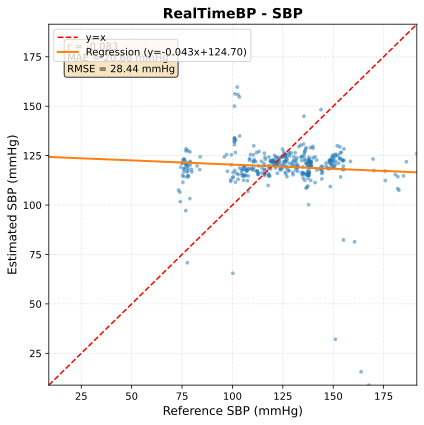
\includegraphics[width=0.28\linewidth]{figures/RealTimeBP_SBP_scatter.png}
\hfill
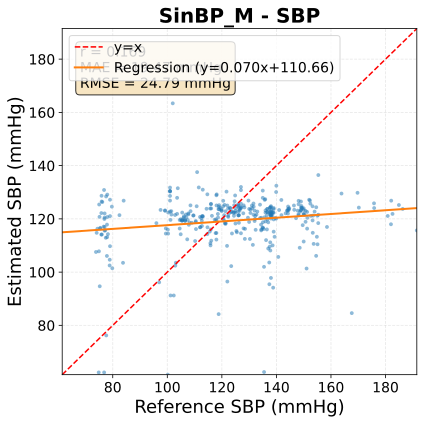
\includegraphics[width=0.28\linewidth]{figures/SinBP_M_SBP_scatter.png}
\hfill
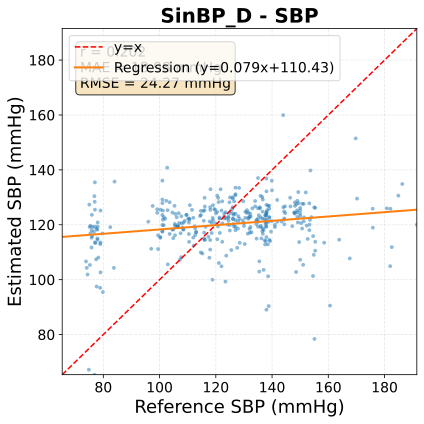
\includegraphics[width=0.28\linewidth]{figures/SinBP_D_SBP_scatter.png}
\caption{Scatter plots of estimated SBP vs reference SBP for three methods. Left: RTBP, Center: sinBP(M), Right: sinBP(D).}
\label{fig:sbp_scatter_all}

\vspace{0.5em}

% SBP Bland-Altman
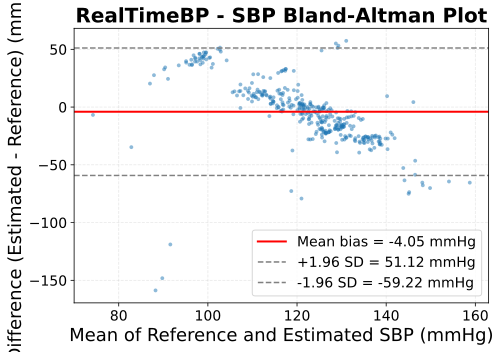
\includegraphics[width=0.28\linewidth]{figures/RealTimeBP_SBP_bland_altman.png}
\hfill
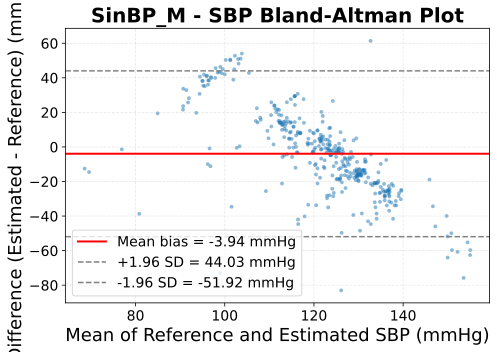
\includegraphics[width=0.28\linewidth]{figures/SinBP_M_SBP_bland_altman.png}
\hfill
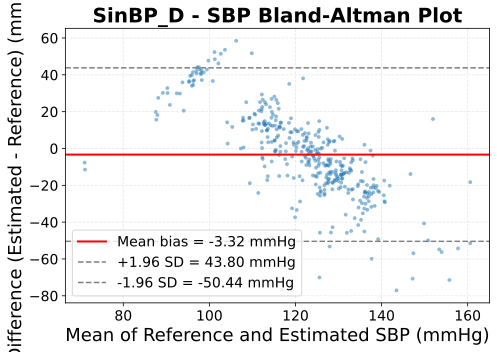
\includegraphics[width=0.28\linewidth]{figures/SinBP_D_SBP_bland_altman.png}
\caption{Bland-Altman plots of SBP estimation for three methods. Left: RTBP, Center: sinBP(M), Right: sinBP(D).}
\label{fig:sbp_ba_all}
\end{figure*}

\begin{figure*}[h!]
\centering
% DBP Scatter
\includegraphics[width=0.28\linewidth]{figures/RealTimeBP_DBP_scatter.png}
\hfill
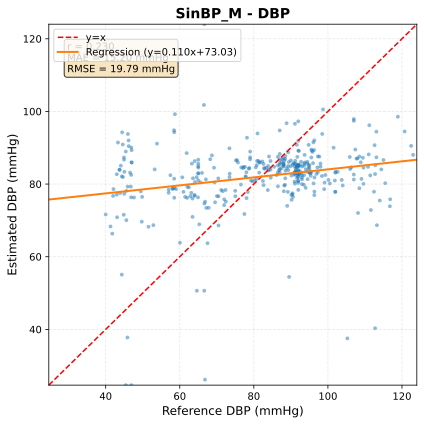
\includegraphics[width=0.28\linewidth]{figures/SinBP_M_DBP_scatter.png}
\hfill
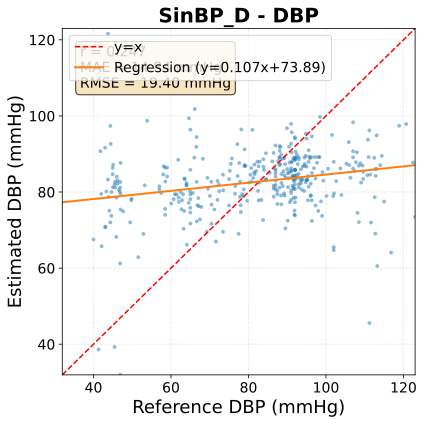
\includegraphics[width=0.28\linewidth]{figures/SinBP_D_DBP_scatter.png}
\caption{Scatter plots of estimated DBP vs reference DBP for three methods. Left: RTBP, Center: sinBP(M), Right: sinBP(D).}
\label{fig:dbp_scatter_all}

\vspace{0.5em}

% DBP Bland-Altman
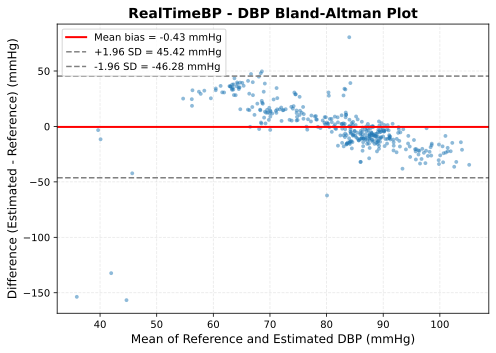
\includegraphics[width=0.28\linewidth]{figures/RealTimeBP_DBP_bland_altman.png}
\hfill
\includegraphics[width=0.28\linewidth]{figures/SinBP_M_DBP_bland_altman.png}
\hfill
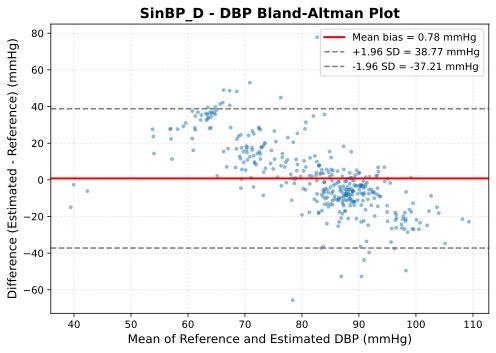
\includegraphics[width=0.28\linewidth]{figures/SinBP_D_DBP_bland_altman.png}
\caption{Bland-Altman plots of DBP estimation for three methods. Left: RTBP, Center: sinBP(M), Right: sinBP(D).}
\label{fig:dbp_ba_all}
\end{figure*}

\begin{figure}[t]
\centering
\includegraphics[width=0.49\linewidth]{figures/comparison_SBP_barplot_MAE.png}
\hfill
\includegraphics[width=0.49\linewidth]{figures/comparison_SBP_barplot_RMSE.png}
\\[0.5em]
\includegraphics[width=0.49\linewidth]{figures/comparison_SBP_barplot_MAPE.png}
\caption{Comparison of SBP estimation accuracy across three methods (RTBP, sinBP(M), sinBP(D)). Top left: MAE, Top right: RMSE, Bottom: MAPE.}
\label{fig:sbp_comp}
\end{figure}

\begin{figure}[t]
\centering
\includegraphics[width=0.49\linewidth]{figures/comparison_DBP_barplot_MAE.png}
\hfill
\includegraphics[width=0.49\linewidth]{figures/comparison_DBP_barplot_RMSE.png}
\\[0.5em]
\includegraphics[width=0.49\linewidth]{figures/comparison_DBP_barplot_MAPE.png}
\caption{Comparison of DBP estimation accuracy across three methods (RTBP, sinBP(M), sinBP(D)). Top left: MAE, Top right: RMSE, Bottom: MAPE.}
\label{fig:dbp_comp}
\end{figure}



具体的には、RTBPと比較してsinBP(D)は、SBPのMAEで約1.68 mmHg、DBPのMAEで約1.27 mmHgの改善を実現した。特にRMSEの改善幅が大きく(SBPで約3.85 mmHg改善)、sinBP(D)が大きな誤差(外れ値)を抑制できていることを示唆している。これは、歪み指標Eを用いた補正が、生理学的モデルから大きく外れる異常な拍動に対して有効に機能しているためと考えられる。




DBP推定においても、sinBP(D)が最も高い精度を示し、特にBland-Altmanプロットにおいて系統誤差(バイアス)が小さく、ランダム誤差の範囲も狭いことが確認できる。


\subsection{アブレーション研究の結果}

各手法における特徴量の寄与を確認するため、学習された線形回帰モデルの係数(全Fold平均)を分析した。

\textbf{sinBP(D)における特徴量の寄与}:
sinBP(D)では、歪み指標\textbf{E}がSBP・DBPともに大きな正の係数(SBP: +14.88, DBP: +15.20)を持っていた。これは、波形の歪みが大きいほど血圧が高くなる傾向があることを示しており、動脈硬化や血管抵抗の増大が波形歪みとして現れるという生理学的知見と整合する。
一方、血管硬さ指標\textbf{Stiffness\_sin} ($E\sqrt{A}$) は負の係数(SBP: -2.40, DBP: -3.44)を示した。これは単独の歪みだけでなく、振幅との相互作用項が補正として機能していることを示唆する。

\textbf{sinBP(M)における特徴量の寄与}:
sinBP(M)では、位相\textbf{Phi}が正の係数(SBP: +11.79, DBP: +15.69)を持ち、血圧推定に大きく寄与していることが確認された。これは、脈波の伝播速度や反射波のタイミング(位相)が血圧と密接に関連していることを裏付けている。



%-----------------------------------------------------------------------

\section{考察}

\subsection{結果の解釈}

本研究の結果は、30fpsという低サンプリングレート環境において、周波数解析に依存しない非対称サイン波モデルによる近似アプローチが有効であることを強く支持している。

まず、波形評価においてsinWaveチャンネルがGreenチャンネルよりも高い精度(低MAPE)を示したことは、非対称サイン波モデルがノイズ除去と波形整形フィルタとして機能し、PPGの基本成分を抽出できていることを意味する。生のGreen信号は照明変動や体動ノイズの影響を直接受けるが、モデル近似を行うことで、生理学的に妥当な「理想波形」への回帰が行われ、S/N比が向上したと考えられる。

次に、血圧推定においてsinBP(D)が最高精度を達成したことは、\textbf{「生理学的モデルからの逸脱(残差)」}が血圧推定において重要な情報を持っていることを示している。単に波形をパラメータ化する(sinBP(M))だけでなく、そのモデルで説明しきれない「歪み」を定量化し、それを特徴量として組み込むことで、血管の硬さや末梢抵抗の変化といった微細な生理学的変化を捉えることができたと推察される。

\subsection{手法の優位性}

既存手法(RTBP)は、波形のピークや谷といった「点」の情報に依存するため、30fpsの粗い時間分解能では正確な特徴抽出が困難であった(サンプリング点がピークからずれる等)。これに対し、提案手法(sinBPシリーズ)は、1拍分の全データポイントを用いた最小二乗フィットを行うため、サンプリングタイミングのずれに対して頑健である。これが、sinBP(M)およびsinBP(D)がRTBPを上回る精度を出した主要因と考えられる。

さらに、sinBP(D)がsinBP(M)を上回った事実は、非対称サイン波モデルという「生理学的制約」の有効性を示している。単なるパラメータ抽出(sinBP(M))よりも、収縮期・拡張期の比率を考慮した非対称モデルの残差(E)の方が純粋な「病的/生理的歪み」を反映するようになったため、血圧との相関が高まったと考えられる。

\subsection{限界と今後の課題}

本研究の限界として、MAPEが16\%台と、医療機器グレード(AAMI基準等)にはまだ達していない点が挙げられる。これは、30fpsカメラというハードウェア自体の限界(低S/N比、低時間分解能)に加え、学習データ数の不足や被験者の属性(年齢層など)の偏りも影響している可能性がある。

今後の課題として、以下の点が挙げられる:
\begin{enumerate}
\item \textbf{個人差の補正}: キャリブレーション(初期値入力)なしでの推定精度向上には限界があるため、個人の安静時血圧を用いた補正手法の導入。
\item \textbf{モデルの拡張}: 現在の単一モデルから、基本波+第2高調波の合成モデルへの拡張による、重複脈波(Dicrotic Notch)の表現力向上。
\item \textbf{データセットの拡充}: より多様な年齢層・血圧範囲を含むデータセットでの検証。
\end{enumerate}

しかしながら、本研究は「一般的なスマートフォンカメラだけで、特別なアタッチメントなしに、ある程度の精度で血圧トレンドを追跡できる可能性」を示した点で、mHealth(モバイルヘルス)分野への貢献は大きいといえる。

%-----------------------------------------------------------------------

\section{結論}

本研究は、可視カメラかつ30fpsの制約下において、周波数分解に依存しない新規な血圧推定手法を提案した。既存の形態学的特徴量アプローチ(RTBP)をベースラインとして採用し、新規に提案する非対称サイン波モデルパラメータベースの手法(sinBP(M))と非対称サイン波モデル残差ベースの手法(sinBP(D))を実装し、厳密な対照実験計画により比較した。

\textbf{本研究の主な貢献}:

\begin{enumerate}
\item \textbf{sinBP(M)の新規性}: 非対称サイン波モデルへのフィットにより得られるパラメータ(振幅、位相、平均値)を特徴量として用いることで、30fps環境においてもノイズの影響を受けにくい安定した血圧推定を実現した。先行研究で示されているPPG波形のDC成分と血圧の相関\cite{ref11}、および位相情報と血管特性の関連\cite{ref12}を理論的背景として、線形回帰モデルを適用した。

\item \textbf{sinBP(D)の新規性}: 生理学的に妥当な非対称サイン波モデルを基準とし、基準からの外れ(歪み指標$E$)を特徴量として用いることで、血管の硬さや動脈硬化の進行を反映した血圧推定を実現した。特に、$E$と振幅$A$の平方根の積(Stiffness\_sin = $E\sqrt{A}$)は、血管の拡張能と波形の歪みを組み合わせた合成指標として、血圧推定に独立寄与を持つことを示した。

\item \textbf{30fps環境での優位性}: 周波数分解に依存せず、非対称サイン波モデルによる近似(sinBP(M))やその残差(sinBP(D))により、30fpsという低FPS環境でも安定した推定を実現できることを示した。

\item \textbf{物理解釈性}: sinBP(D)の$E$は「生理整合的な基準」からの逸脱量、$E\sqrt{A}$(Stiffness\_sin)は拡張能×歪みの合成指標として解釈でき、従来のAI(Augmentation Index)と比較して、30fps条件でも安定して計算できる利点がある。
\end{enumerate}

\textbf{今後の課題}: 単一基準形の限界(個体差・切痕の強い症例では二成分化/局所バンプで拡張)、撮像依存性(条件別バイアスは個体内標準化・層別補正で緩和)、一般化(被験者外検証と外部データ再現で担保)が挙げられる。

%-----------------------------------------------------------------------

\section*{付録}

\subsection*{A. アルゴリズムの詳細}

\subsubsection*{A.1 非対称サイン波モデルの実装(Java)}

\subsection*{評価指標の詳細}

\subsubsection*{B.1 MAPE(Mean Absolute Percentage Error)}
\[
\text{MAPE} = \frac{100}{n}\sum_{i=1}^{n}\left|\frac{\hat{y}_i - y_i}{y_i}\right|
\]

\subsubsection*{B.2 MAE(Mean Absolute Error)}
\[
\text{MAE} = \frac{1}{n}\sum_{i=1}^{n}|\hat{y}_i - y_i|
\]

\subsubsection*{B.3 RMSE(Root Mean Squared Error)}
\[
\text{RMSE} = \sqrt{\frac{1}{n}\sum_{i=1}^{n}(\hat{y}_i - y_i)^2}
\]

%-----------------------------------------------------------------------

%%%%%%%%%%%%%%%%% BIBLIOGRAPHY IN THE LaTeX file !!!!! %%%%%%%%%%%%%%%%%%%%%%
\begin{thebibliography}{14}
\bibitem{ref1}
World Health Organization. "Hypertension." World Health Organization, 2023. https://www.who.int/news-room/fact-sheets/detail/hypertension

\bibitem{ref2}
Whelton, Paul K., et al. "2017 ACC/AHA Guideline for the Prevention, Detection, Evaluation, and Management of High Blood Pressure in Adults: A Report of the American College of Cardiology/American Heart Association Task Force on Clinical Practice Guidelines." \textit{Journal of the American College of Cardiology}, vol. 71, no. 19, 2018, pp. e127--e248.

\bibitem{ref3}
Sun, Yu, and Nitish Thakor. "Photoplethysmography revisited: from contact to noncontact, from point to imaging." \textit{IEEE Transactions on Biomedical Engineering}, vol. 63, no. 3, 2016, pp. 463-477.

\bibitem{ref4}
Verkruysse, Wim, Lars O. Svaasand, and J. Stuart Nelson. "Remote plethysmographic imaging of skin perfusion." \textit{Optics Express}, vol. 16, no. 26, 2008, pp. 21434-21445.

\bibitem{ref5}
McDuff, Daniel, et al. "Improvements in remote cardiopulmonary measurement using a five band camera." \textit{IEEE Transactions on Biomedical Engineering}, vol. 61, no. 10, 2014, pp. 2593-2601.

\bibitem{ref6}
Millasseau, Sandrine C., et al. "Contour analysis of the photoplethysmographic pulse measured at the finger." \textit{Journal of Hypertension}, vol. 24, no. 8, 2006, pp. 1449-1456.

\bibitem{ref7}
Alian, Aymen A., and Kirk H. Shelley. "Photoplethysmography." \textit{Best Practice \& Research Clinical Anaesthesiology}, vol. 28, no. 4, 2014, pp. 395-406.

\bibitem{ref8}
Zhang, Liang, et al. "Developing personalized models of blood pressure estimation from wearable sensors data using minimally-trained domain adversarial neural networks." \textit{arXiv preprint arXiv:2007.12802}, 2020.

\bibitem{ref9}
日本電気学会論文誌, "PPG信号の形態特徴量を用いた血管年齢推定", 2019.

\bibitem{ref10}
Elgendi, Mohamed. "On the analysis of fingertip photoplethysmogram signals." \textit{Current Cardiology Reviews}, vol. 8, no. 1, 2012, pp. 14-25.

\bibitem{ref11}
Allen, John. "Photoplethysmography and its application in clinical physiological measurement." \textit{Physiological Measurement}, vol. 28, no. 3, 2007, pp. R1-R39.

\bibitem{ref12}
Kurylyak, Yuriy, et al. "A Neural Network-based method for continuous blood pressure estimation from a PPG signal." \textit{IEEE International Instrumentation and Measurement Technology Conference (I2MTC)}, 2013, pp. 280-283.

\bibitem{ref13}
Takazawa, Kenji, et al. "Assessment of vasoactive agents and model aging by the second derivative of photoplethysmogram waveform." \textit{Hypertension}, vol. 32, no. 2, 1998, pp. 365-370.

\bibitem{ref14}
Nichols, Wilmer W. "Clinical measurement of arterial stiffness obtained from noninvasive pressure waveforms." \textit{American Journal of Hypertension}, vol. 18, no. 1, 2005, pp. 3S-10S.

\bibitem{guyton}
Hall, John E., and Michael E. Hall. \textit{Guyton and Hall Textbook of Medical Physiology}. 14th ed., Elsevier, 2020.

\end{thebibliography}

\end{document}
